% This example is meant to be compiled with lualatex or xelatex
% The theme itself also supports pdflatex
\PassOptionsToPackage{unicode}{hyperref}
\documentclass[xcolor=dvipsnames, aspectratio=1610, 12pt]{beamer}

% Warning, if another latex run is needed
% \usepackage[aux]{rerunfilecheck}

% just list chapters and sections in the toc, not subsections or smaller
\setcounter{tocdepth}{1}

%------------------------------------------------------------------------------
%------------------------------ Fonts, Unicode, Language ----------------------
%------------------------------------------------------------------------------
\usepackage{fontspec}
\defaultfontfeatures{Ligatures=TeX}  % -- becomes en-dash etc.

% german language
\usepackage{polyglossia}
\setdefaultlanguage{german}

% for english abstract and english titles in the toc
\setotherlanguages{english}

% intelligent quotation marks, language and nesting sensitive
\usepackage[autostyle]{csquotes}

% microtypographical features, makes the text look nicer on the small scale
\usepackage{microtype}

% colors and stuff
\usepackage{xcolor}
\usepackage[most]{tcolorbox}
\tcbset{on line,
        boxsep=4pt, left=0pt,right=0pt,top=0pt,bottom=0pt,
        colframe=white,colback=SpringGreen,
        highlight math style={enhanced}
        }
\newtcolorbox{mybox}[3][]
{
  colframe = #2!25,
  colback = #2!20,
  coltitle = #2!20!black,
  title = {#3},
  #1
}
%\colorlet{Green!40}
%------------------------------------------------------------------------------
%------------------------ Math Packages and settings --------------------------
%------------------------------------------------------------------------------

\usepackage{amsmath}
\usepackage{amssymb}
\usepackage{mathtools}
\usepackage{bbold}

% Enable Unicode-Math and follow the ISO-Standards for typesetting math
\usepackage[
  math-style=ISO,
  bold-style=ISO,
  sans-style=italic,
  nabla=upright,
  partial=upright,
]{unicode-math}
\setmathfont{Latin Modern Math}

% nice, small fracs for the text with \sfrac{}{}
\usepackage{xfrac}


%------------------------------------------------------------------------------
%---------------------------- Numbers and Units -------------------------------
%------------------------------------------------------------------------------

\usepackage[
  locale=DE,
  separate-uncertainty=true,
  per-mode=symbol-or-fraction,
]{siunitx}
\sisetup{math-micro=\text{µ},text-micro=µ}
% \sisetup{tophrase={{ to }}}
%------------------------------------------------------------------------------
%-------------------------------- tables  -------------------------------------
%------------------------------------------------------------------------------

\usepackage{booktabs}       % \toprule, \midrule, \bottomrule, etc

%------------------------------------------------------------------------------
%-------------------------------- graphics -------------------------------------
%------------------------------------------------------------------------------

\usepackage{graphicx}
%\usepackage{rotating}
\usepackage{grffile}
\usepackage{tikz}
\usepackage{circuitikz}
\usepackage{tikz-feynman}
\usepackage{subcaption}

% allow figures to be placed in the running text by default:
\usepackage{scrhack}
\usepackage{float}
\floatplacement{figure}{htbp}
\floatplacement{table}{htbp}

% keep figures and tables in the section
\usepackage[section, below]{placeins}

% smileys
\usepackage{MnSymbol,wasysym}

%------------------------------------------------------------------------------
%---------------------- customize list environments ---------------------------
%------------------------------------------------------------------------------

\usepackage{enumitem}
\usepackage{listings}
\usepackage{hepunits}

\usepackage{pdfpages}
%------------------------------------------------------------------------------
%------------------------------ Bibliographie ---------------------------------
%------------------------------------------------------------------------------

\usepackage[
  backend=biber,   % use modern biber backend
  autolang=hyphen, % load hyphenation rules for if language of bibentry is not
                   % german, has to be loaded with \setotherlanguages
                   % in the references.bib use langid={en} for english sources
]{biblatex}
\addbibresource{references.bib}  % the bib file to use
\DefineBibliographyStrings{german}{andothers = {{et\,al\adddot}}}  % replace u.a. with et al.


% Load packages you need here
% \usepackage{polyglossia}
% \setmainlanguage{german}

\usepackage{csquotes}


% \usepackage{amsmath}
% \usepackage{amssymb}
% \usepackage{mathtools}

\usepackage{hyperref}
\usepackage{bookmark}

% load the theme after all packages

\usetheme[
  showtotalframes, % show total number of frames in the footline
]{tudo}

% Put settings here, like
\unimathsetup{
  math-style=ISO,
  bold-style=ISO,
  nabla=upright,
  partial=upright,
  mathrm=sym,
}

% \setbeamertemplate{itemize item}{\scriptsize$\blacktriangleright$}
% \setbeamertemplate{itemize subitem}{\scriptsize$\blacktriangleright$}

%Titel:
\title{The LHCb SciFi Tracker}
%Autor
\author[N.Breer]{\textbf{Nils Breer}}
%Lehrstuhl/Fakultät
\institute{16. Terascale Detector Workshop}
%Titelgrafik muss ich einfueren!!!
%\titlegraphic{\includegraphics[width=0.3\textwidth]{content/Bilder/interferenz.jpg}}
\date{21.02.2024}

\begin{document}
\maketitle

\begin{frame}\frametitle{Overview}
  % \begin{columns}
  %   \begin{column}[c]{0.48\textwidth}
  \begin{itemize}
    \item $\bullet$\, The SciFi Detector Upgrade
    \item $\bullet$\, Importance of the SciFi and Alignment
    \item $\bullet$\, Understanding first alignments on 2022 data
  \end{itemize}
\end{frame}

\begin{frame}\frametitle{Importance of alignments}
  \begin{itemize}
    \item $\bullet$\, Alignment is part of the LHCb trigger system
    \item $\bullet$\, Physics performance tied to alignment performance
    \item $\bullet$\, with optimal alignment:
    \begin{itemize}
      \item $\bullet$\, \to\, remove systematic biases for asymmetry measurements
      \item $\bullet$\, best possible mass resolution
    \end{itemize}
  \end{itemize}
  \begin{figure}
      \includegraphics[width=0.9\textwidth]{logos/dataflow.png}%
    % \caption{Hits on tracks in x-direction with run 256145 data on 20000 ents using 9 minimum hits against 11 minimum hits.}
  \end{figure}
\end{frame}

\begin{frame}\frametitle{LHCb upgraded with the SciFi}
  \begin{columns}
    \begin{column}[c]{0.48\textwidth}
      \begin{figure}
        \includegraphics[width=\textwidth]{logos/upgrade_lhcb.png}
        % \caption{Visualization of the SciFi tracking stations.}
      \end{figure}
    \end{column}
    \begin{column}{0.48\textwidth}
      \begin{itemize}
        \item $\bullet$\, Consists of 3 stations: T1, T2, T3
        \item $\bullet$\, 4 layers per station: X1, U, V, X2
	      \item $\bullet$\, replaces former IT and OT to cope with the increased instantaneous luminosity
	      \item $\bullet$\, crucial part of tracking system
      \end{itemize}
      \includegraphics[width=0.5\textwidth]{plots/track.png}
    \end{column}
  \end{columns}
\end{frame}

\begin{frame}\frametitle{The Scintillating Fibre Tracker}
  \begin{columns}
    \begin{column}[c]{0.48\textwidth}
      \begin{figure}
        \includegraphics[width=0.9\textwidth]{logos/scifi.png}
        % \caption{Visualization of the SciFi tracking stations.}
      \end{figure}
    \end{column}
    \begin{column}{0.48\textwidth}
      \begin{itemize}
        \item $\bullet$\, Front two stations have 5 modules per side
        \item $\bullet$\, Back station has 6 modules on each side
        \item $\bullet$\, U, V layers have a $\mp 5 \deg$ stereo angle respectively
        \item $\bullet$\, \to\, used for determining y-position of tracks by comparing hitposition at different angles
      \end{itemize}
    \end{column}
  \end{columns}
\end{frame}

\begin{frame}\frametitle{SciFi terminology}
  layers are divided into two halves commonly labeled as A-side and C-side
  % \begin{itemize}
  %   \item $\bullet$\, layers are divided into two halves commonly labeled as A-side and C-side
  % \end{itemize}
  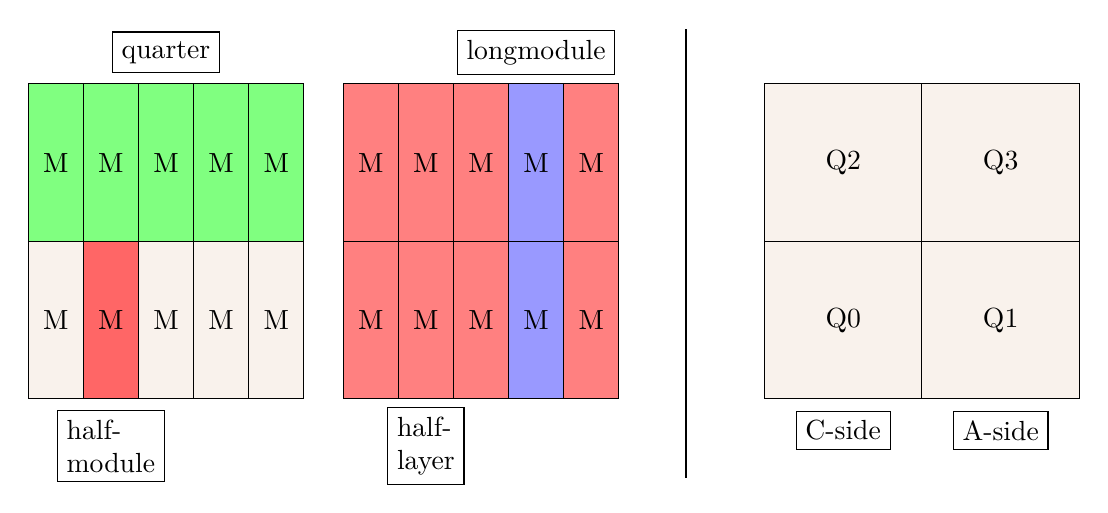
\begin{tikzpicture}
% first quarter
  \node[rectangle,
      draw = black,
      % text = ,
      fill = brown!10!white,
      minimum width = 0.7cm,
      minimum height = 2cm] (r) at (0,0) {M};

  \node[rectangle,
      draw = black,
      % text = half-module,
      fill = red!60!white,
      minimum width = 0.7cm,
      minimum height = 2cm] (r) at (0.7,0) {M};

  \node[rectangle,
      draw = black,
      % text = ,
      fill = brown!10!white,
      minimum width = 0.7cm,
      minimum height = 2cm] (r) at (1.4,0) {M};

  \node[rectangle,
      draw = black,
      % text = ,
      fill = brown!10!white,
      minimum width = 0.7cm,
      minimum height = 2cm] (r) at (2.1,0) {M};

  \node[rectangle,
      draw = black,
      % text = ,
      fill = brown!10!white,
      minimum width = 0.7cm,
      minimum height = 2cm] (r) at (2.8,0) {M};

% second quarter
\node[rectangle,
    draw = black,
    % text = ,
    fill = red!50!white,
    minimum width = 0.7cm,
    minimum height = 2cm] (r) at (4,0) {M};

\node[rectangle,
    draw = black,
    % text = ,
    fill = red!50!white,
    minimum width = 0.7cm,
    minimum height = 2cm] (r) at (4.7,0) {M};

\node[rectangle,
    draw = black,
    % text = ,
    fill = red!50!white,
    minimum width = 0.7cm,
    minimum height = 2cm] (r) at (5.4,0) {M};

\node[rectangle,
    draw = black,
    % text = ,
    fill = blue!40!white,
    minimum width = 0.7cm,
    minimum height = 2cm] (r) at (6.1,0) {M};

\node[rectangle,
    draw = black,
    % text = ,
    fill = red!50!white,
    minimum width = 0.7cm,
    minimum height = 2cm] (r) at (6.8,0) {M};

% third quarter
\node[rectangle,
    draw = black,
    % text = ,
    fill = green!50!white,
    minimum width = 0.7cm,
    minimum height = 2cm] (r) at (0,2) {M};

\node[rectangle,
    draw = black,
    % text = quarter,
    fill = green!50!white,
    minimum width = 0.7cm,
    minimum height = 2cm] (r) at (0.7,2) {M};

\node[rectangle,
    draw = black,
    % text = ,
    fill = green!50!white,
    minimum width = 0.7cm,
    minimum height = 2cm] (r) at (1.4,2) {M};

\node[rectangle,
    draw = black,
    % text = ,
    fill = green!50!white,
    minimum width = 0.7cm,
    minimum height = 2cm] (r) at (2.1,2) {M};

\node[rectangle,
    draw = black,
    % text = ,
    fill = green!50!white,
    minimum width = 0.7cm,
    minimum height = 2cm] (r) at (2.8,2) {M};

% fourth quarter
\node[rectangle,
    draw = black,
    % text = ,
    fill = red!50!white,
    minimum width = 0.7cm,
    minimum height = 2cm] (r) at (4,2) {M};

\node[rectangle,
    draw = black,
    % text = ,
    fill = red!50!white,
    minimum width = 0.7cm,
    minimum height = 2cm] (r) at (4.7,2) {M};

\node[rectangle,
    draw = black,
    % text = ,
    fill = red!50!white,
    minimum width = 0.7cm,
    minimum height = 2cm] (r) at (5.4,2) {M};

\node[rectangle,
    draw = black,
    % text = ,
    fill = blue!40!white,
    minimum width = 0.7cm,
    minimum height = 2cm] (r) at (6.1,2) {M};

\node[rectangle,
    draw = black,
    % text = ,
    fill = red!50!white,
    minimum width = 0.7cm,
    minimum height = 2cm] (r) at (6.8,2) {M};

\node[draw, align=left] at (1.4, 3.4) {quarter};
\node[draw, align=left] at (0.7, -1.6) {half-\\module};
\node[draw, align=left] at (4.7, -1.6) {half-\\layer};
\node[draw, align=left] at (6.1, 3.4) {longmodule};

% draw a vertical line to seperate the plots
\draw[thick] (8,-2) -- (8,3.7);

% label quarters
\node[rectangle,
    draw = black,
    % text = Q2,
    fill = brown!10!white,
    minimum width = 2cm,
    minimum height = 2cm] (r) at (10,0) {Q0};

\node[rectangle,
    draw = black,
    % text = Q3,
    fill = brown!10!white,
    minimum width = 2cm,
    minimum height = 2cm] (r) at (12,0) {Q1};

\node[rectangle,
    draw = black,
    % text = Q0,
    fill = brown!10!white,
    minimum width = 2cm,
    minimum height = 2cm] (r) at (10,2) {Q2};

\node[rectangle,
    draw = black,
    % text = Q1,
    fill = brown!10!white,
    minimum width = 2cm,
    minimum height = 2cm] (r) at (12,2) {Q3};

\node[draw, align=left] at (10, -1.4) {C-side};
\node[draw, align=left] at (12, -1.4) {A-side};

\end{tikzpicture}

\end{frame}

\begin{frame}\frametitle{What is Alignment and why do we need it?}
  \begin{columns}
    \begin{column}[c]{0.48\textwidth}
      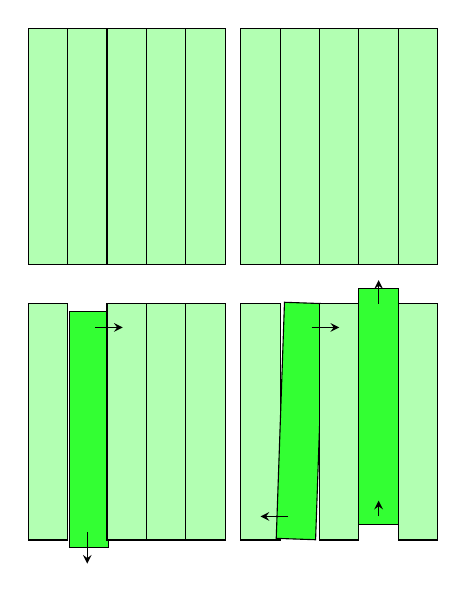
\begin{tikzpicture}
  % this is the ideal detector
  \node[rectangle,
      draw = black,
      % text = ,
      fill = green!30!white,
      minimum width = 0.5cm,
      minimum height = 3cm] (r) at (0,0) {};
  \node[rectangle,
      draw = black,
      % text = ,
      fill = green!80!white,
      minimum width = 0.5cm,
      minimum height = 3cm] (r) at (0.525,-0.1) {};
  \node[rectangle,
      draw = black,
      % text = ,
      fill = green!30!white,
      minimum width = 0.5cm,
      minimum height = 3cm] (r) at (1,0) {};
  \node[rectangle,
      draw = black,
      % text = ,
      fill = green!30!white,
      minimum width = 0.5cm,
      minimum height = 3cm] (r) at (1.5,0) {};
  \node[rectangle,
      draw = black,
      % text = ,
      fill = green!30!white,
      minimum width = 0.5cm,
      minimum height = 3cm] (r) at (2,0) {};

  \node[rectangle,
      draw = black,
      % text = ,
      fill = green!30!white,
      minimum width = 0.5cm,
      minimum height = 3cm] (r) at (2.7,0) {};
  \node[rectangle,
      draw = black,
      % text = ,
      fill = green!80!white,
      rotate around = {-2:(3.2,0)},
      minimum width = 0.5cm,
      minimum height = 3cm] (r) at (3.2,-0.1) {};
  % \draw (2.7,0) -- (5.7,0);
  \node[rectangle,
      draw = black,
      % text = ,
      fill = green!30!white,
      minimum width = 0.5cm,
      minimum height = 3cm] (r) at (3.7,0) {};
  \node[rectangle,
      draw = black,
      % text = ,
      fill = green!80!white,
      minimum width = 0.5cm,
      minimum height = 3cm] (r) at (4.2,0.2) {};
  \node[rectangle,
      draw = black,
      % text = ,
      fill = green!30!white,
      minimum width = 0.5cm,
      minimum height = 3cm] (r) at (4.7,0) {};

% now below it the physical detector
\node[rectangle,
    draw = black,
    % text = ,
    fill = green!30!white,
    minimum width = 0.5cm,
    minimum height = 3cm] (r) at (0,3.5) {};
\node[rectangle,
    draw = black,
    % text = ,
    fill = green!30!white,
    minimum width = 0.5cm,
    minimum height = 3cm] (r) at (0.5,3.5) {};
\node[rectangle,
    draw = black,
    % text = ,
    fill = green!30!white,
    minimum width = 0.5cm,
    minimum height = 3cm] (r) at (1,3.5) {};
\node[rectangle,
    draw = black,
    % text = ,
    fill = green!30!white,
    minimum width = 0.5cm,
    minimum height = 3cm] (r) at (1.5,3.5) {};
\node[rectangle,
    draw = black,
    % text = ,
    fill = green!30!white,
    minimum width = 0.5cm,
    minimum height = 3cm] (r) at (2,3.5) {};

\node[rectangle,
    draw = black,
    % text = ,
    fill = green!30!white,
    minimum width = 0.5cm,
    minimum height = 3cm] (r) at (2.7,3.5) {};
\node[rectangle,
    draw = black,
    % text = ,
    fill = green!30!white,
    minimum width = 0.5cm,
    minimum height = 3cm] (r) at (3.2,3.5) {};
\node[rectangle,
    draw = black,
    % text = ,
    fill = green!30!white,
    minimum width = 0.5cm,
    minimum height = 3cm] (r) at (3.7,3.5) {};
\node[rectangle,
    draw = black,
    % text = ,
    fill = green!30!white,
    minimum width = 0.5cm,
    minimum height = 3cm] (r) at (4.2,3.5) {};
\node[rectangle,
    draw = black,
    % text = ,
    fill = green!30!white,
    minimum width = 0.5cm,
    minimum height = 3cm] (r) at (4.7,3.5) {};

% draw arrows indicating the movement
% x and y translation
\draw [-stealth] (0.6,1.2) -- (0.95,1.2);
\draw [-stealth] (0.5,-1.4) -- (0.5,-1.8);

% rotation
\draw [-stealth] (3.35,1.2) -- (3.7,1.2);
\draw [-stealth] (3.05,-1.2) -- (2.7,-1.2);
% single translation
\draw [-stealth] (4.2,1.5) -- (4.2,1.8);
\draw [-stealth] (4.2,-1.2) -- (4.2,-1);

\end{tikzpicture}

    \end{column}
    \begin{column}[c]{0.48\textwidth}
      \begin{itemize}
        \item $\bullet$\, top: ideal detector, bottom: physical detector
        \item $\bullet$\, Surveys are used to find the rotation and position of each detector component
        \item $\bullet$\, Are used as starting positions for software alignment
        \item $\bullet$\, Building tracks accurately requires positions in reconstruction to be as similar as possible to real positions
      \end{itemize}
    \end{column}
  \end{columns}
\end{frame}

\begin{frame}\frametitle{The survey: what is it and the different types}
  \begin{columns}
    \begin{column}[c]{0.48\textwidth}
      $\bullet$\, measure distance of some points on the detector with a laser
      \begin{figure}
        \centering
        \includegraphics[width=\textwidth]{logos/survey.png}
        % \caption{}
      \end{figure}
    \end{column}
    \begin{column}[c]{0.48\textwidth}
      \begin{itemize}
        \item $\bullet$\, 2022: photogrammetry was recorded in assembly hall \to\, not quite perfect
        \item $\bullet$\, 2023: photogrammetry will be recorded in cavern
        \item $\bullet$\, relative angles and positions between points are compared to simulation
        \item $\bullet$\, layer survey: performed in the cavern on the layer in  the front in closed state (both halves together)
        \item $\bullet$\, module survey: performed inside assembly hall using reflective stickers keeping track of all positions
        % \item $\bullet$\, layer survey: performed in the cavern on the layer n the front in closed state (both halves together)
      \end{itemize}
    \end{column}
  \end{columns}
\end{frame}

\begin{frame}\frametitle{Alignment: track fits with the Kalman Filter}
  \begin{columns}
    \begin{column}[c]{0.4\textwidth}
      \begin{figure}
        \centering
        \includegraphics[width=0.72\textwidth]{logos/kalman.png}
        % \caption{Alignment with Kalman Filter.}
      \end{figure}
    \end{column}
    \begin{column}[c]{0.55\textwidth}
      \begin{itemize}
        \item $\bullet$\, Use survey information as starting point
        \item $\bullet$\, aligning the detector by minimizing the residuals of the track hits
        \item $\bullet$\, basically a $\chi^2$ minimization problem with alignment parameters $\alpha$
        \item $\bullet$\, Why Kalman Filter?
        \begin{itemize}
          \item $\bullet$\, easily models material interactions as well as multiple scattering
        \end{itemize}
        \item $\bullet$\, propagation of nodes, minimization, smooth error sizes by back propagation
      \end{itemize}
    \end{column}
  \end{columns}
\end{frame}

\begin{frame}\frametitle{Alignment versions in use}
  \begin{columns}
    \begin{column}[c]{0.33\textwidth}
      \centering
      \includegraphics[width=\textwidth]{logos/LHCb-FIGURE-2022-018/Run251342Preliminary_BestLong_chi2_per_ndof.pdf}
    \end{column}
    \begin{column}[c]{0.33\textwidth}
      \begin{itemize}
        \item $\bullet$\, V1: First ever SciFi alignments for the upgraded LHCb detector
	      \item $\bullet$\, Using early tracks from comissioning
        \item $\bullet$\, use full length modules
        \item $\bullet$\, alignable degrees of freedom: Tx Rz (x translation, rotation around z \to beam pipe axis)
      \end{itemize}
    \end{column}
    \begin{column}[c]{0.33\textwidth}
      \begin{itemize}
        \item $\bullet$\, V2: Updated alignment version with what we learned from V1 %(hard work from detector experts)
        \item $\bullet$\, aligned using half modules
        \item $\bullet$\, uses newest time alignment
      \end{itemize}
    \end{column}
  \end{columns}
\end{frame}

\begin{frame}\frametitle{Hit distribution per quarter in V1 and V2 alignment}
  \begin{itemize}
    \item $\bullet$\, Improvements to V2 visible on A-side, losing some performance on C-side
    \item $\bullet$\, Alignment performance difference in each quarter \to\, seperately analyse quarters!
    \item $\bullet$\, $\chi2$ per quarter can provide more insights about alignment performance in each detector part
  \end{itemize}
  \begin{mybox}{green}{}
    \begin{itemize}
      \item $\bullet$\, analysis of each quarter seperately makes finding possible issues easier
    \end{itemize}
  \end{mybox}
  \begin{figure}
      \includegraphics[width=0.8\textwidth]{logos/v1_v2.png}%
      % \includegraphics[width=0.45\textwidth]{logos/hit_dist_v2.png}%
  \end{figure}
\end{frame}

\begin{frame}\frametitle{Track hits comparison of V2 and simulation}
\begin{mybox}{green}{}
  \begin{itemize}
    \item $\bullet$\, MC: hits on \textbf{reconstructed} tracks fill whole detector
    \item $\bullet$\, data: filling tracks into A-side \to\, good!
  \end{itemize}
\end{mybox}
\begin{mybox}{orange}{}
  \begin{itemize}
    \item \to\, scan C-side quarters for possible issues in distinct layers
  \end{itemize}
\end{mybox}
  \begin{columns}
    \begin{column}[c]{0.48\textwidth}
      \begin{figure}
        \centering
        \includegraphics[width=0.6\textwidth]{logos/nodeXY_MC.pdf}%
      \end{figure}
    \end{column}
    % \begin{column}[c]{0.48\textwidth}
    %   \begin{figure}
    %     \centering
    %     \includegraphics[width=0.6\textwidth]{tuples_out/combining_2D_nodeXY_v2.pdf}%
    %   \end{figure}
    % \end{column}
  \end{columns}
\end{frame}

\begin{frame}\frametitle{New Q0 positions in T2X2 layer}
  \begin{itemize}
    \item $\bullet$\, Changes based on V2 alignment positions
    \item $\bullet$\, test incremental shifts of position/rotation until we found an improvement
    \item $\bullet$\, rotations are with regard to the local frame of the module
    \item $\bullet$\, positions: translations relative to the nominal position for each module
    \item $\bullet$\, V2 alignment has only few tracks in Q0 because parts of the SciFi are too far out of alignment
  \end{itemize}
  \begin{figure}
    \includegraphics[width=0.26\textwidth]{logos/2D_nodeXY_v2_7_left.pdf}%
    \includegraphics[width=0.26\textwidth]{logos/2D_nodeXY_quartermean_7_left.pdf}%
    \includegraphics[width=0.26\textwidth]{plots/problem_layer.png}%
  \end{figure}
\end{frame}

\begin{frame}\frametitle{Summary}
  \begin{itemize}
    \item $\bullet$\, Trying to solve a puzzle on unexpected lower number of alignment tracks on the C-side
    \item $\bullet$\, Source of complications: SciFi parts too far out of alignment to be correctly updated
    \item $\bullet$\, \to\, Varying the positions and rotations of Q0 modules yielded more tracks in more modules
    \item $\bullet$\, Feeding this back into tracking alignment to get the fine tuning right
    \item $\bullet$\, new survey/photogrammetry in progress to improve alignment starting conditions this year
  \end{itemize}
  \textbf{Thank you for your attention!}
\end{frame}

\end{document}
